\section*{Summary in simple words}
\begin{itemize}[leftmargin=1.4em,itemsep=2pt]
\item Some passengers, such as wheelchair users, should enter a lift before other people. We call this \emph{priority-first boarding}. We asked: how much longer do the other people wait because of this rule, and how can a lift controller make the rule work better?
\item We built a computer model of lifts. It works in seconds, with real speeds, door times and boarding times. We checked it against the standard lift formula. The difference is less than 2\%.
\item We ran the model 31,680 times: three buildings, steady and rising-and-falling demand, five control methods, and two kinds of priority passenger (one who takes one place, and a wheelchair-like passenger who takes three places and boards slowly).
\item \textbf{Result 1.} With normal call buttons, the priority rule costs other people almost nothing when the lifts can carry everyone (never more than 3.3 seconds). In busy periods it helps priority passengers a lot (about 80 seconds) and costs the others about 14 seconds.
\item \textbf{Result 2.} With destination control (you enter your floor on a keypad and are sent to one car), priority at the door does nothing in normal operation. Our new rule lets the controller use the priority label when it chooses the car. Priority passengers then wait about one third less, and the others wait 1 to 4 seconds more.
\item \textbf{Result 3.} Wheelchair-like passengers need more space and time. This makes everyone wait longer, much more than the boarding order does.
\item \textbf{Result 4.} Two ways to calculate the average waiting time agree about which control method is better.
\end{itemize}

\section*{Words used in this paper}
\begin{longtable}{@{}p{.27\linewidth}p{.68\linewidth}@{}}
\toprule Word & Meaning\\\midrule\endhead
\bottomrule\endlastfoot
Lift car & The box that carries people up and down.\\
Lift group & Several cars that serve the same floors and work together.\\
Landing & The place on a floor where people wait for a car.\\
Landing call & A person presses the UP or DOWN button on a landing.\\
Group controller & The computer program that chooses which car answers each call.\\
Round trip & A car leaves the main lobby, takes people up, and comes back to the lobby.\\
Handling capacity & The largest number of people the lift group can carry in five minutes in the morning rush.\\
Demand level ($x$) & How many people arrive, compared with the handling capacity. $x=1.0$ (100\%) means exactly as many people arrive as the lifts can carry. $x=1.3$ (130\%) means 30\% too many.\\
Waiting time & The time from when a person arrives at the landing until the doors of their car begin to open.\\
Served passenger & A person who boarded a car before the simulation ended.\\
Served-only average & The average waiting time of served passengers only. People who are still waiting at the end are left out. This is the usual measure.\\
Capped average wait ($R_{600}$) & The average waiting time of \emph{all} counted passengers, where any wait longer than 600 seconds is counted as 600 seconds.\\
Priority passenger & A person who is allowed to board first.\\
Wheelchair-like passenger & A priority passenger who takes three places in the car and needs three times the normal time to enter or leave.\\
Replication & One repeat of the same test with new random passengers.\\
\end{longtable}

\section{Introduction}\label{sec:intro}

Engineers use computer simulation to design lift systems and to compare group controllers. Design guides describe simulation as a normal tool, next to the classical hand calculation \cite{cibse2025,iso8100,barney2016}. Research papers on lift control also use simulation to decide which controller is better \cite{siikonen1993,kim1995,crites1998,utgoff2012,wan2024}. The usual measure is the average waiting time.

An average is only useful if we know which people it includes. When a building is quiet, every person gets a car before the simulation ends, so the average includes everyone. When a building is very busy, queues grow. Some people are still waiting when the simulation stops. We do not know their full waiting time, but we know it is long. If the average includes only the people who boarded, it leaves out the people with the worst service. The same problem is well known in medical studies, where some patients are still being followed when the study ends. There, researchers use a \emph{restricted mean}: an average in which every time is capped at a fixed limit \cite{royston2013}. Simulation textbooks also warn that the length of the observation period changes what an average means \cite{law2015}. Lift studies rarely say how they treat people who are still waiting.

The same question matters for boarding priority. Some passengers, for example wheelchair users, should board before other people. The standard EN~81-70 sets rules for accessible lifts \cite{en8170}. Recent work finds such passengers with cameras and serves them first \cite{han2024}. If a car has room for everyone, the boarding order changes nothing. Other people can only lose time when a car is full and leaves someone behind. Queueing theory has a ``conservation law'' for simple queues with one server: priority moves waiting time from one group to another, but the total stays the same \cite{kleinrock1965,schrage1970}. A lift group is not such a simple queue. The boarding order changes how full each car is, where it stops and where it goes next. So we must measure the effect.

This paper asks three questions:
\begin{enumerate}[itemsep=2pt]
\item How much does priority-first boarding cost other passengers and give priority passengers? How does this change with demand, with the controller, and when the priority passenger needs more space and time?
\item Destination control sends each passenger to one fixed car. Can it serve priority passengers better if it uses the priority label when it chooses the car, and not only at the door?
\item Does the usual served-only average rank controllers in the same order as an average that includes everyone?
\end{enumerate}

The paper makes four contributions:
\begin{enumerate}[itemsep=2pt]
\item An open lift simulator that works in seconds, with real car movement, door times and boarding times, passengers of different sizes, five group controllers and optional priority boarding. Its round-trip times differ from the classical formula by less than 2\% (Section~\ref{sec:validation}).
\item A measurement of the cost and the gain of priority-first boarding for each controller, from 50\% to 130\% of handling capacity and in demand that rises and falls, for a simple priority passenger and for a wheelchair-like passenger (Section~\ref{sec:priority}).
\item A new priority-aware destination control rule, in two versions, and a test of what it gives priority passengers and what it costs the others (Section~\ref{sec:dcsp}).
\item A test plan in which every counted passenger is watched for at least 900 seconds, so that the capped average wait of all passengers is exact, and a check of whether the usual average gives the same ranking of controllers (Sections~\ref{sec:design} and~\ref{sec:disagreement}).
\end{enumerate}
The test plan, the simulator, all results and the analysis programs are public \cite{dataset}. The model is described following the STRESS reporting guidelines \cite{monks2019} (\ref{app:stress}).

\section{Related work}\label{sec:related}

\paragraph{Lift traffic calculation and simulation} Classical lift design calculates the round-trip time of a car in the morning rush. From it come the interval between cars and the handling capacity \cite{barney2016}. The calculation assumes that every car leaves the lobby equally full and that all floors have the same number of people. Monte Carlo simulation removes these assumptions and has been checked against the formula \cite{alsharif2012}. Simulation is now part of standard design practice \cite{cibse2025,iso8100}. Simulators also exist for special cases such as hospitals \cite{chu2003} and shafts with several cars \cite{miyamoto2008}. Siikonen showed early that, in heavy traffic, the service level depends strongly on the group controller \cite{siikonen1993}.

\paragraph{Group controllers} Many methods have been proposed: fuzzy rules \cite{kim1995,fernandez2014}, search methods \cite{hamdi2007}, genetic and tabu search \cite{cortes2004,bolat2011,cortes2021}, real-time optimisation \cite{utgoff2012}, reinforcement learning \cite{crites1998,wan2024} and learning from occupancy data \cite{wang2021}. The estimated-time-to-destination (ETD) method gives each call to the car with the lowest total time for the new passenger and for the passengers it delays \cite{smith2002}. Destination control asks each passenger for their floor before they board \cite{sorsa2018}. All of these studies compare controllers by simulated waiting times. We use clear versions of the classical rules, add one controller that knows how many people are waiting, as in occupancy-aware control \cite{wang2021,kimmoon2001}, and propose a priority-aware version of destination control.

\paragraph{Priority and accessibility} Cameras have been used to count waiting passengers \cite{kimmoon2001} and to dispatch cars fairly \cite{yamauchi2019}. Han et al.\ detect passengers with special needs and give them priority \cite{han2024}. EN~81-70 covers access to lifts for people with disabilities \cite{en8170}. In this paper, priority is a simple yes/no label on each passenger. We do not study how the label is obtained.

\paragraph{Averages when some people are still waiting} When observation ends before everyone is served, the average of the observed times is too low. The restricted mean solves this if every person is followed at least up to the cap \cite{royston2013}. We apply this idea to lift waiting times and plan the observation period so that the condition is met.

\section{The lift model}\label{sec:model}

\subsection{Parts of a lift system}
Figure~\ref{fig:system} shows the parts of the model. A building has a main lobby (floor 0) and a number of floors above it. Several lift cars serve all floors. People arrive at a landing, press a call button and wait in a queue. The group controller chooses which car answers each call.

\begin{figure}[htbp]\centering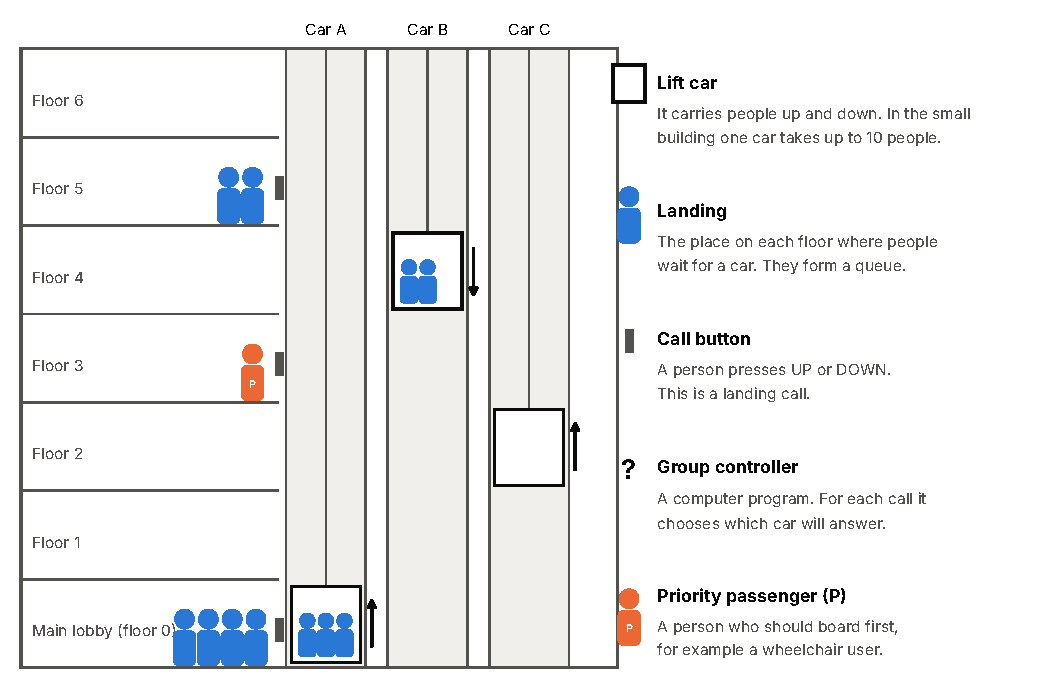
\includegraphics[width=\linewidth]{pic_system.pdf}
\caption{The parts of a lift system in the model. The drawing shows the lobby and six floors of a building with three cars. Arrows show the direction of each car. The orange figure marked P is a priority passenger.}\label{fig:system}\end{figure}

\subsection{Buildings}
We model three office buildings (Table~\ref{tab:buildings}). Each has one main lobby and 50 people on every floor above it. The distance between floors is 3.6~m. A car accepts passengers up to a \emph{boarding limit} of 80\% of its rated load, the usual assumption in lift design \cite{barney2016}.

\begin{table}[htbp]\centering
\caption{The three buildings. The last three columns come from the classical calculation with cars filled to the boarding limit: round-trip time (RTT), interval between cars, and five-minute handling capacity (HC5).}\label{tab:buildings}
\small
\begin{tabular}{@{}lrrrrrrrrr@{}}
\toprule
 & Floors & Cars & Rated & Limit & Speed & Accel. & RTT & Interval & HC5\\
 & & & (pers.) & (pers.) & (m/s) & (m/s$^2$) & (s) & (s) & (pers.)\\\midrule
B1 (small) & 10 & 3 & 13 & 10 & 1.6 & 1.0 & 120.1 & 40.0 & 74.9\\
B2 (medium) & 16 & 4 & 17 & 13 & 2.5 & 1.0 & 154.5 & 38.6 & 101.0\\
B3 (large) & 24 & 6 & 21 & 16 & 3.5 & 1.2 & 187.8 & 31.3 & 153.4\\
\bottomrule
\end{tabular}

\smallskip\parbox{.97\linewidth}{\footnotesize ``Floors means floors above the lobby. The buildings hold 500, 800 and 1,200 people, so HC5 is 15.0\%, 12.6\% and 12.8\% of the people in the building. The classical formula is $\mathrm{RTT}=2Ht_v+(S+1)t_s+2Pt_p$, where $P$ is the number of people in the car, $S$ the expected number of stops, $H$ the highest floor reached, $t_v$ the time to pass one floor at full speed, $t_s$ the extra time for one stop and $t_p$ the time for one person to enter or leave \cite{barney2016}.}
\end{table}

\subsection{How a car moves and stops}
Figure~\ref{fig:stop} shows one trip and one stop. A car speeds up, travels at full speed and slows down. The time for a trip of length $D$ is
\begin{equation}
t_f(D)=t_{sd}+\begin{cases} D/v + v/a, & \text{if } D\ge v^2/a,\\ 2\sqrt{D/a}, & \text{if } D<v^2/a,\end{cases}
\label{eq:flight}
\end{equation}
where $v$ is the full speed, $a$ is the acceleration and $t_{sd}=0.5$~s is a short delay before the car starts. The second line is for short trips where the car never reaches full speed. At a stop, the doors open (2.0~s), people leave one by one (1.2~s each), people enter one by one (1.2~s each) and the doors close (3.0~s).

\begin{figure}[htbp]\centering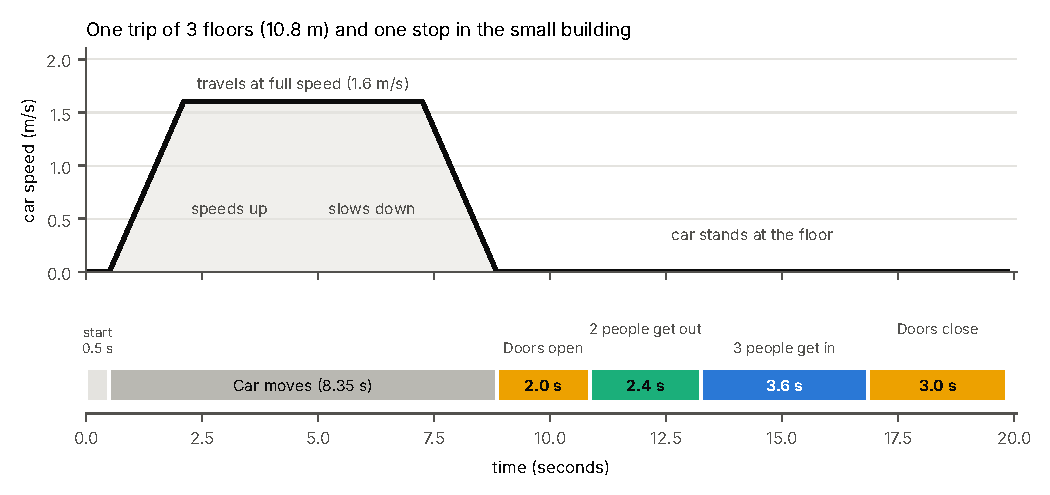
\includegraphics[width=\linewidth]{pic_stop.pdf}
\caption{One trip of three floors and one stop in building B1. Top: the speed of the car. Bottom: what happens and how long each step takes. The trip takes 8.85~s and the stop takes 11.0~s.}\label{fig:stop}\end{figure}

A car keeps moving in one direction while it has people to deliver or calls to answer in that direction. Then it turns round. A moving car can accept a new stop only if it still has enough distance to slow down. A car with nothing to do returns to the main lobby. A full car does not stop for landing calls.

\subsection{Passengers}
Passengers arrive at random moments at a steady average rate (a Poisson process). There are three kinds of passenger: \emph{incoming} (from the lobby to an upper floor), \emph{outgoing} (from an upper floor to the lobby) and \emph{interfloor} (between two upper floors). Upper floors are chosen with equal chance. We use three traffic patterns:
\begin{itemize}[itemsep=1pt]
\item \emph{Up-peak} (morning): 85\% incoming, 10\% outgoing, 5\% interfloor.
\item \emph{Lunch}: 40\% incoming, 40\% outgoing, 20\% interfloor.
\item \emph{Down-peak} (evening): 5\% incoming, 85\% outgoing, 10\% interfloor.
\end{itemize}
The demand level compares the arrival rate $\lambda$ (people per second) with the handling capacity of Table~\ref{tab:buildings}:
\begin{equation}
x=\frac{300\,\lambda}{\mathrm{HC5}}.
\label{eq:load}
\end{equation}
So $x=1$ means that, in five minutes, exactly as many people arrive as the lifts can carry in the morning rush. We use the same scale for all three patterns.

Besides steady demand, we also test demand that rises and falls, as in a real morning (Figure~\ref{fig:ramp}). Demand starts at 50\% of handling capacity, rises in a straight line to a peak after 30 minutes, falls back to 50\% after 60 minutes and stays there. The peak is 100\%, 115\%, 130\% or 150\% of handling capacity, with the up-peak mix.

\begin{figure}[htbp]\centering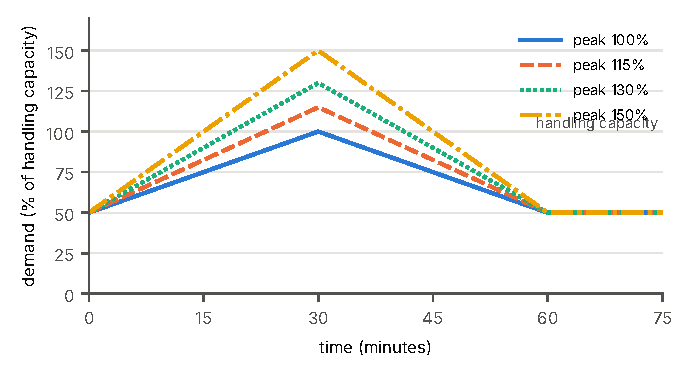
\includegraphics[width=.62\linewidth]{pic_ramp.pdf}
\caption{Rising and falling demand. The four lines are the four peak levels. The grey line marks handling capacity. Above the grey line, more people arrive than the lifts can carry, but only for a limited time.}\label{fig:ramp}\end{figure}

Each passenger also gets a random number between 0 and 1. If the number is below the \emph{priority share} $s$, the passenger is a priority passenger. These numbers come from a separate random source. So the passengers, their times and their floors are exactly the same whatever share we choose. We use two kinds of priority passenger:
\begin{itemize}[itemsep=1pt]
\item \emph{Simple priority passenger} (15\% of passengers): takes one place and boards at normal speed. This stands for people who should board first but need no extra space, such as older people.
\item \emph{Wheelchair-like passenger} (5\% of passengers): takes three places in the car and needs three times the normal time to enter and to leave (3.6~s). These two values are assumptions, not measurements. If such a passenger does not fit into the free space of a car, the people behind may board, and the passenger waits for another car.
\end{itemize}

\subsection{The group controllers}
All controllers use the same cars. They differ only in how they choose a car (Table~\ref{tab:controllers}). With the first four, a person presses UP or DOWN and may board any car that opens its doors for that direction. With destination control, a person enters their floor on a keypad, is told which car to use, and boards only that car.

\begin{table}[htbp]\centering
\caption{The group controllers in simple words.}\label{tab:controllers}
\small\begin{tabular}{@{}p{.10\linewidth}p{.22\linewidth}p{.60\linewidth}@{}}
\toprule Short name & Full name & How it chooses a car\\\midrule
NC & Nearest car & The closest car that is moving towards the call, or is free.\\
ETA & Estimated time of arrival & The car that can reach the call soonest. The controller plans each car's stops and adds the travel and stop times.\\
ETD & Estimated time to destination & Like ETA, but it also adds the delay that the new stop causes to people already using that car \cite{smith2002}.\\
ETDQ & ETD with queue knowledge & Like ETD, but the controller knows how many people wait behind each call (for example from a camera). It counts every waiting person, avoids cars without enough room, and chooses again when the queue grows.\\
DCS & Destination control & Each passenger gives their floor first. The controller picks the car with the lowest sum of this passenger's total trip time and the delay to that car's other passengers. It avoids cars that would be too full.\\
DCS-P1, DCS-P0 & Priority-aware destination control (new) & Like DCS, but it uses the priority label when it chooses the car (Section~\ref{sec:dcspmodel}).\\
\bottomrule\end{tabular}
\end{table}

In detail, NC scores a car $N+2-d$ if it moves towards the call in the same direction, $N+1-d$ if it is free or moves towards the call in the other direction, and 1 if it moves away ($N$ floors above the lobby, distance $d$ floors); the highest score wins. ETA, ETD, ETDQ and DCS plan each car's stops with Eq.~\eqref{eq:flight} and a stop time of $t_o+t_c$ plus the boarding time of each expected person. ETDQ multiplies the arrival time by the number of people waiting and adds 30~s for each place that the car is expected to lack. DCS adds 600~s when the planned load would pass the boarding limit. If a car cannot take the people at a landing, their call is given to another car. These are clear textbook versions of well-known rules. They are not copies of commercial products.

\subsection{Priority-aware destination control}\label{sec:dcspmodel}
With normal destination control, priority can act only at the door, among the people who were sent to the same car. A priority passenger who is sent to a car that is far away must still wait for that car. The new rule changes two things:
\begin{enumerate}[itemsep=2pt]
\item \emph{Choosing the car.} When the controller chooses a car for a priority passenger, it does not count the other (general) passengers who wait at the same landing for that car, because the priority passenger will board before them. So a car that looks full to a general passenger can still be chosen for a priority passenger.
\item \emph{Moving people early.} If the priority passenger makes the car too full, the controller at once sends the general passengers who arrived last at that landing to other cars. They do not wait at the door for a car that they cannot enter.
\end{enumerate}
There are two versions. In DCS-P1 the controller still counts the delay that the priority passenger causes to all other passengers of that car. In DCS-P0 it ignores this delay, so the priority passenger simply gets the car with the shortest trip. DCS-P0 is stronger for the priority passenger and harder on the others. Both versions were developed on separate practice runs that are not part of the results.

\subsection{The two boarding rules}
Figure~\ref{fig:boarding} shows the two rules. With \emph{first come, first served} (FCFS), people board in the order they arrived. With \emph{priority-first boarding} (PFB), priority passengers board first, and then the other people in the order they arrived. Except for DCS-P1 and DCS-P0, no controller uses the priority label when it chooses a car, so priority works only through the boarding order.

\begin{figure}[htbp]\centering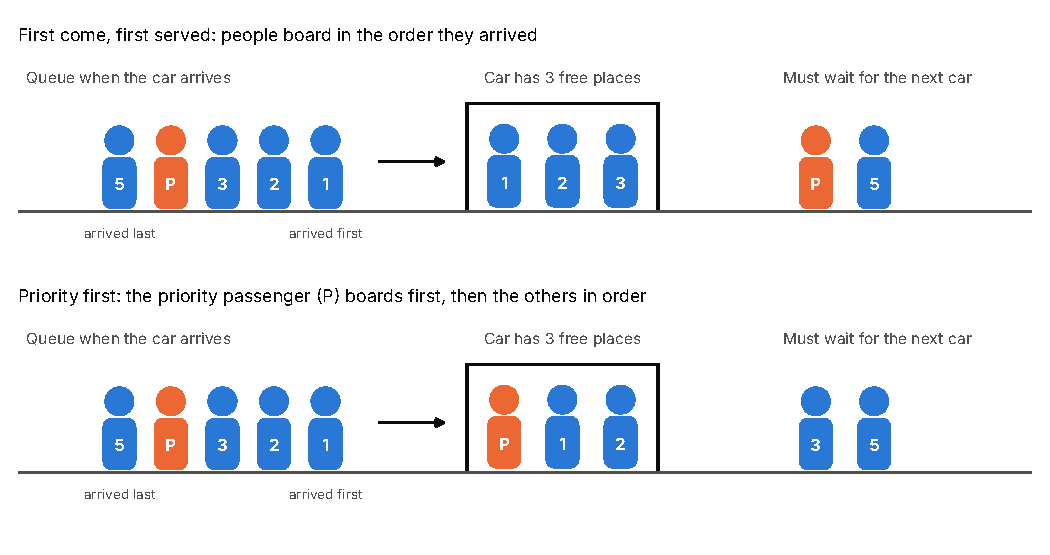
\includegraphics[width=\linewidth]{pic_boarding.pdf}
\caption{The two boarding rules. Five people wait; the numbers show the order in which they arrived, and P is a priority passenger who arrived fourth. The car has three free places. With priority-first boarding, passenger P boards and passenger 3 must wait for the next car.}\label{fig:boarding}\end{figure}

\subsection{Program and checks}
The simulator is written in Python 3.13 with NumPy. It is event-driven: it jumps from one event (a person arrives, a car arrives, doors open, boarding ends, doors close) to the next. Before the main tests we ran automatic checks. They confirm that nobody boards before arriving, boards twice or leaves a car without boarding; that a car never carries more than its limit; that people only board a car going their way; that destination-control passengers board only their own car; that the same input always gives the same output; that no car keeps moving between floors without opening its doors; that the boarding rule changes nothing when there are no priority passengers; and that DCS-P1 equals DCS when there are no priority passengers. In a further check of 39,588 trips, no ride was shorter than the physical minimum from Eq.~\eqref{eq:flight}.

\section{The test plan}\label{sec:design}

\subsection{Situations and repeats}
There are 66 situations for the three buildings:
\begin{itemize}[itemsep=1pt]
\item \emph{Steady demand}: 3 traffic patterns $\times$ 6 demand levels ($x=0.5$, 0.7, 0.85, 1.0, 1.15, 1.3) in each building (54 situations).
\item \emph{Rising and falling demand}: 4 peak levels in each building (12 situations).
\end{itemize}
Each situation is repeated 20 times with new random passengers. In each repeat, every controller and every boarding setting receives \emph{exactly the same passengers}. This method is called common random numbers \cite{law2015}. It means that any difference in results comes from the controller or the boarding rule, not from luck.

The five standard controllers (NC, ETA, ETD, ETDQ, DCS) are run with four settings: FCFS and PFB with simple priority passengers, and FCFS and PFB with wheelchair-like passengers. DCS-P1 and DCS-P0 are run with PFB for both kinds of priority passenger. In total there are $66\times20\times(5\times4+2\times2)=31{,}680$ runs. We wrote the plan and fixed the program before the runs. No run was removed or repeated.

\subsection{Who is counted, and for how long}
Figure~\ref{fig:window} shows the timing. People arrive from 0 to 4,500~s. We count only the people who arrive between 300 and 3,600~s. The first 300~s are a start-up period, because the model starts with empty cars at the lobby. People keep arriving after 3,600~s so that the building stays busy, but they are not counted. We stop watching at $T=4{,}500$~s. So every counted passenger is watched for at least 900~s.

\begin{figure}[htbp]\centering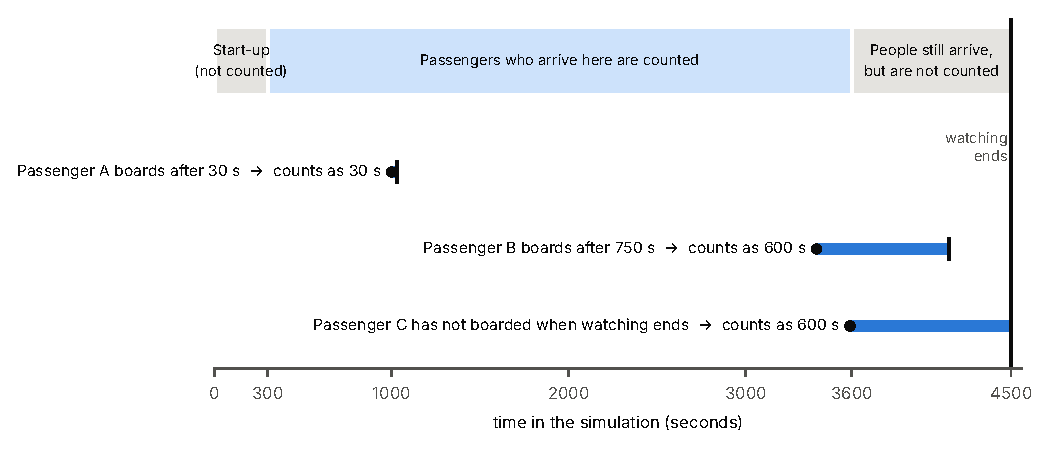
\includegraphics[width=\linewidth]{pic_window.pdf}
\caption{Who is counted and how waiting time is counted. Dots show when a passenger arrives and vertical marks show when they board. In the capped average wait $R_{600}$, a wait above 600~s counts as 600~s. Because every counted passenger is watched for at least 900~s, we always know whether their wait was above 600~s.}\label{fig:window}\end{figure}

\subsection{Measures}
Passenger $i$ arrives at time $a_i$ and boards at time $b_i$ (the moment the doors of their car begin to open). The observed waiting time is
\begin{equation}
W_i=\begin{cases} b_i-a_i, & \text{if the passenger boards before } T,\\ T-a_i, & \text{if the passenger is still waiting at } T.\end{cases}
\label{eq:wait}
\end{equation}
Our main measure is the \emph{capped average wait} over all counted passengers $P$:
\begin{equation}
R_{600}=\frac{1}{|P|}\sum_{i\in P}\min(W_i,\,600).
\label{eq:rmwt}
\end{equation}
In words: take every counted passenger, replace any wait longer than 600~s by 600~s, and take the average. This value is exact, because every passenger is watched for at least 900~s. The usual measure is the \emph{served-only average}:
\begin{equation}
\mathrm{AWT}_{\mathrm{served}}=\frac{1}{|P_b|}\sum_{i\in P_b}W_i,
\label{eq:awt}
\end{equation}
where $P_b$ contains only the counted passengers who boarded before $T$. The two measures differ in two ways: the served-only average leaves out people who are still waiting, and it has no cap. To separate these two effects we also calculate the capped average over served passengers only, $R_{600}^{\mathrm{served}}$. We also report the share of passengers served, and capped averages with caps of 300~s and 900~s. All measures are calculated for all passengers, for priority passengers and for the other (``general'') passengers.

\subsection{Comparisons}
\emph{Priority cost and gain.} For each situation, controller and kind of priority passenger, we take the same 20 passenger streams and subtract the FCFS result from the PFB result. We do this for priority passengers and for the other (general) passengers.

\emph{Priority-aware destination control.} We compare DCS with door-only priority, DCS-P1 and DCS-P0, each against DCS with FCFS boarding.

\emph{Agreement of measures.} For each situation and each of the ten pairs of standard controllers, we ask which controller is better according to each measure. If two measures give opposite answers, the pair is a \emph{disagreement}. If both answers are also statistically clear, it is a \emph{clear disagreement}.

\emph{Uncertainty.} For every difference we give a 95\% interval from a paired bootstrap: the 20 repeats are re-sampled 2,000 times. A difference is ``clear'' when its interval does not include zero. The intervals show the effect of random passengers in the model. They do not show how well the model matches a real building, and they are not corrected for the large number of comparisons.

\section{Results}\label{sec:results}

\subsection{Check against the classical formula}\label{sec:validation}
First we checked the simulator. We ran pure incoming traffic at $x=1.3$, five repeats per building, with the NC and ETD controllers. At this demand every car leaves the lobby filled to the boarding limit, which is what the classical formula assumes. We measured the time between two lobby departures of the same car. Table~\ref{tab:rtt} compares this with the formula. The differences are between $-0.2\%$ and $+1.9\%$. The largest are in building B3, where the cars are too fast to reach full speed between two neighbouring floors; the classical formula is known to be less exact in that case \cite{barney2016,alsharif2012}.

\begin{table}[htbp]\centering
\caption{Round-trip time (s) from the simulator and from the classical formula.}\label{tab:rtt}
\small\begin{tabular}{@{}llrrrr@{}}
\toprule Building & Controller & Trips & Simulator, mean (SD) & Formula & Difference\\\midrule
B1 & NC & 473 & 119.9 (8.7) & 120.1 & $-0.2\%$\\
B1 & ETD & 472 & 120.3 (8.5) & 120.1 & $+0.1\%$\\
B2 & NC & 482 & 155.3 (10.3) & 154.5 & $+0.5\%$\\
B2 & ETD & 483 & 154.9 (10.5) & 154.5 & $+0.3\%$\\
B3 & NC & 587 & 190.5 (10.8) & 187.8 & $+1.4\%$\\
B3 & ETD & 582 & 191.3 (11.2) & 187.8 & $+1.9\%$\\
\bottomrule\end{tabular}
\end{table}

\subsection{The simulator at work}\label{sec:atwork}
Figure~\ref{fig:traj} shows two real runs of building B1 in the morning rush with the ETD controller. On the left, demand is 70\% of handling capacity. The three cars go up and down in turn, and the number of people waiting stays small: never more than 16. All 592 counted passengers are served, and the capped average wait is 15.6~s. On the right, demand is 130\%. The cars make the same kind of trips, always full, but more people arrive than the cars can take. The queue grows without stopping and reaches 325 people. Of 1,068 counted passengers, 96\% are served before watching ends, and the capped average wait is 378~s. This is the difference between a lift group below and above its handling capacity, and it explains all later results.

\begin{figure}[htbp]\centering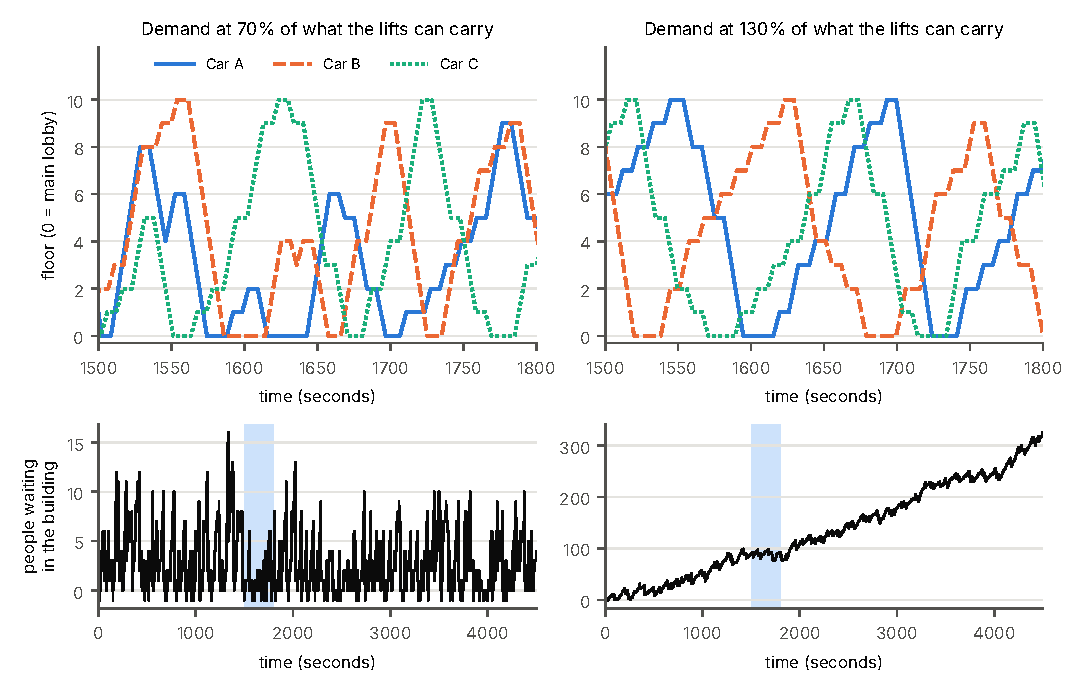
\includegraphics[width=\linewidth]{pic_trajectories.pdf}
\caption{Two runs of the simulator: building B1, up-peak traffic, ETD controller, first-come-first-served boarding. Top: the position of the three cars during five minutes. Bottom: the number of people waiting in the whole building during the full run; the shaded band marks the five minutes shown above. Left: demand below handling capacity. Right: demand above handling capacity.}\label{fig:traj}\end{figure}

\subsection{Waiting time at different demand levels}\label{sec:service}
Figure~\ref{fig:service} shows the waiting time for every steady situation with FCFS boarding and one-place passengers. In up-peak traffic the capped average wait, averaged over buildings and controllers, is 9.6~s at $x=0.5$ and 20.8~s at $x=0.85$. At capacity ($x=1$) it jumps to 48.9~s, and at $x=1.3$ it is 352~s with 95\% of counted passengers served. Lunch and down-peak traffic become overloaded later on this scale.

Below capacity the ETA and ETDQ controllers give the shortest waits (14.7 and 15.0~s at $x=0.5$, against 15.5~s for ETD, 18.9~s for DCS and 19.4~s for NC). At capacity ETDQ is best (38.8~s) and DCS second (41.5~s). Above capacity destination control is clearly best (59.2~s at $x=1.15$ against 109 to 144~s; 105.9~s at $x=1.3$ against 167 to 222~s). This agrees with the general view that destination control carries more people in incoming traffic \cite{barney2016,smith2002}. ETDQ, which knows the queue lengths, is the best call-button controller from $x=0.85$ upward.

\begin{figure}[htbp]\centering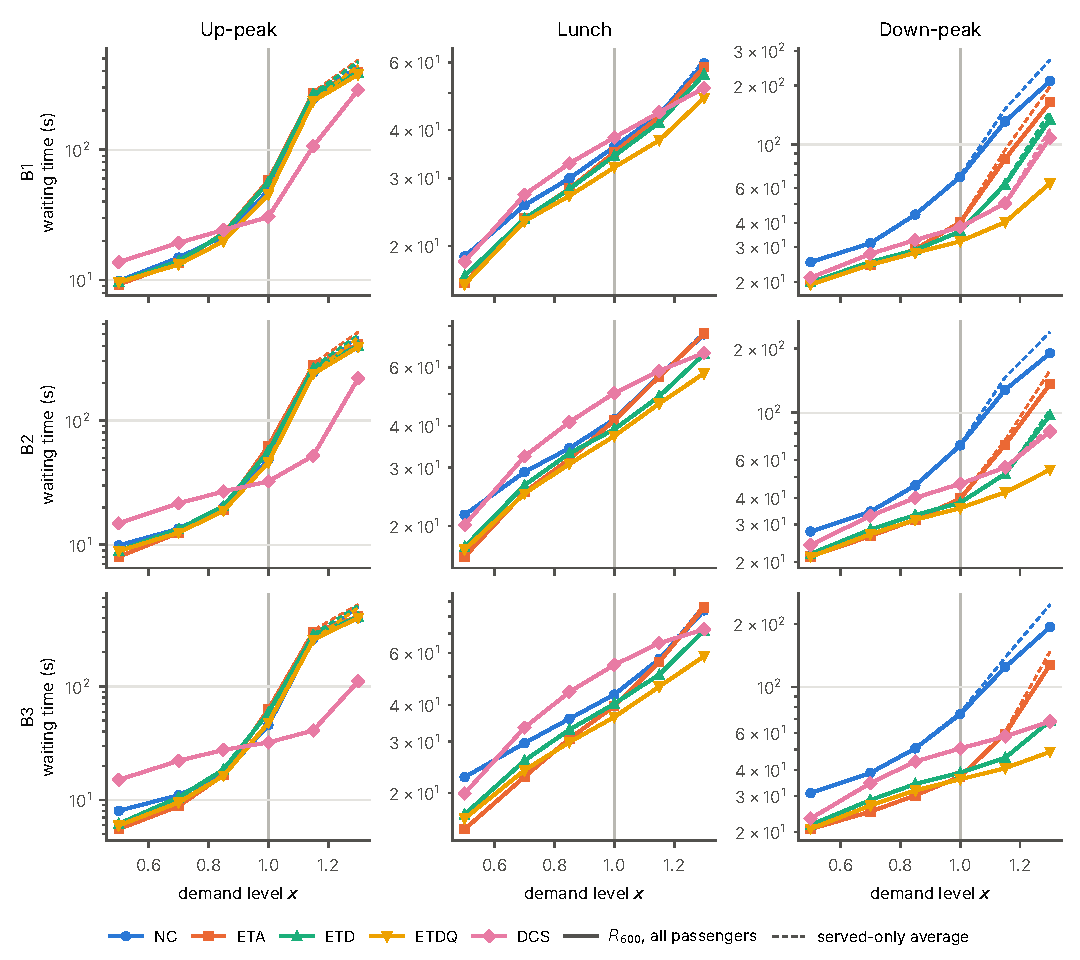
\includegraphics[width=\linewidth]{service_vs_load.pdf}
\caption{Waiting time at each demand level with first-come-first-served boarding. Rows are buildings and columns are traffic patterns. Solid lines with markers: capped average wait $R_{600}$ of all passengers. Dashed lines: served-only average. The vertical scale is logarithmic. The grey vertical line marks handling capacity ($x=1$).}\label{fig:service}\end{figure}

\subsection{What priority-first boarding costs and gives}\label{sec:priority}
Figure~\ref{fig:summary} gives the result in one picture. Table~\ref{tab:prio} and Figure~\ref{fig:priority} give the details for the four call-button controllers. Destination control is treated in Section~\ref{sec:dcsp}.

\begin{figure}[htbp]\centering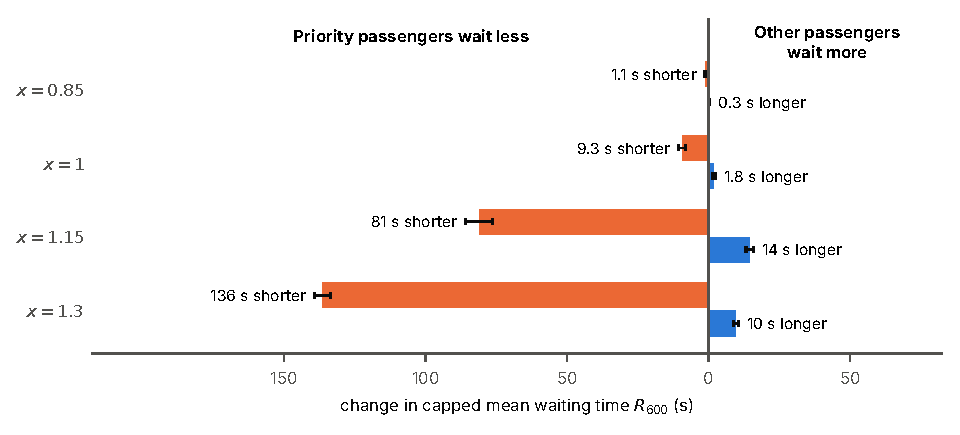
\includegraphics[width=.88\linewidth]{pic_summary.pdf}
\caption{Change in capped average wait when priority-first boarding replaces first-come-first-served boarding, with 15\% simple priority passengers and steady demand. Averages over all buildings, traffic patterns and the five standard controllers.}\label{fig:summary}\end{figure}

\emph{Below capacity the rule is almost free.} With simple priority passengers and call buttons, other passengers wait 0.3~s longer on average at $x=0.85$. The largest cost in any single case below capacity is 3.3~s. Priority passengers also gain little (1.1~s at $x=0.85$), because almost everyone already fits into the first car.

\emph{At capacity the cost is small and the gain is useful.} At $x=1$ other passengers wait 1.8~s longer, and priority passengers wait 9.3~s less (21\% of their wait).

\emph{Above capacity both grow.} At $x=1.15$ other passengers wait 14.5~s longer (11\%) and priority passengers 81.1~s less (63\%). At $x=1.3$ the gain is 136.5~s. The cost at $x=1.3$ (9.7~s) is smaller than at $x=1.15$ only because many general passengers already wait longer than the 600~s cap.

\emph{The cost appears where cars are full.} In steady up-peak traffic the cost is 5.3~s at $x=1$ and 40.2~s at $x=1.15$. In lunch traffic it stays below 2~s at every level. In down-peak it is about 3~s at $x=1.15$ and $x=1.3$.

\emph{Demand that rises and falls.} A short period above capacity is enough to create a cost. With a peak of 100\% the cost is 0.9~s and the gain 2.5~s. With a peak of 115\% they are 4.4~s and 18.7~s; with 130\%, 14.6~s and 76.0~s; with 150\%, 31.4~s and 186.1~s.

\emph{Wheelchair-like passengers.} The pattern is the same, and the gain for the priority passenger is larger: at $x=1$ other passengers wait 3.4~s longer and wheelchair-like passengers 32.0~s less. Below capacity the largest cost in any case is 2.2~s. A separate effect is much bigger than the boarding rule. When 5\% of passengers take three places and board slowly, \emph{everyone} waits longer, with or without priority: 2.9~s longer at $x=0.85$, 21.7~s at $x=1$ and 38.6~s at $x=1.15$, because the cars carry fewer people. A building with many wheelchair users needs more lift capacity; the boarding order is the smaller question.

\begin{table}[htbp]\centering
\caption{Priority-first boarding minus first-come-first-served boarding: average change in capped average wait $R_{600}$ (s) for the four call-button controllers (NC, ETA, ETD, ETDQ) and three buildings. Plus means a longer wait. Steady rows are averages over the three traffic patterns.}\label{tab:prio}
\small\begin{tabular}{@{}lrrrr@{}}
\toprule & \multicolumn{2}{c}{Simple priority (15\%)} & \multicolumn{2}{c}{Wheelchair-like (5\%)}\\
Demand & Others & Priority & Others & Priority\\\midrule
Steady, 50\% & 0.0 & 0.0 & 0.0 & $-0.1$\\
Steady, 70\% & $+0.1$ & $-0.2$ & $+0.1$ & $-0.5$\\
Steady, 85\% & $+0.3$ & $-1.1$ & $+0.4$ & $-3.0$\\
Steady, 100\% & $+1.8$ & $-9.3$ & $+3.4$ & $-32.0$\\
Steady, 115\% & $+14.5$ & $-81.1$ & $+9.1$ & $-118.0$\\
Steady, 130\% & $+9.7$ & $-136.5$ & $+6.7$ & $-155.8$\\
\midrule
Rise and fall, peak 100\% & $+0.9$ & $-2.5$ & $+1.2$ & $-9.4$\\
Rise and fall, peak 115\% & $+4.4$ & $-18.7$ & $+5.5$ & $-49.0$\\
Rise and fall, peak 130\% & $+14.6$ & $-76.0$ & $+16.1$ & $-138.3$\\
Rise and fall, peak 150\% & $+31.4$ & $-186.1$ & $+21.5$ & $-258.3$\\
\bottomrule\end{tabular}
\end{table}

\begin{figure}[htbp]\centering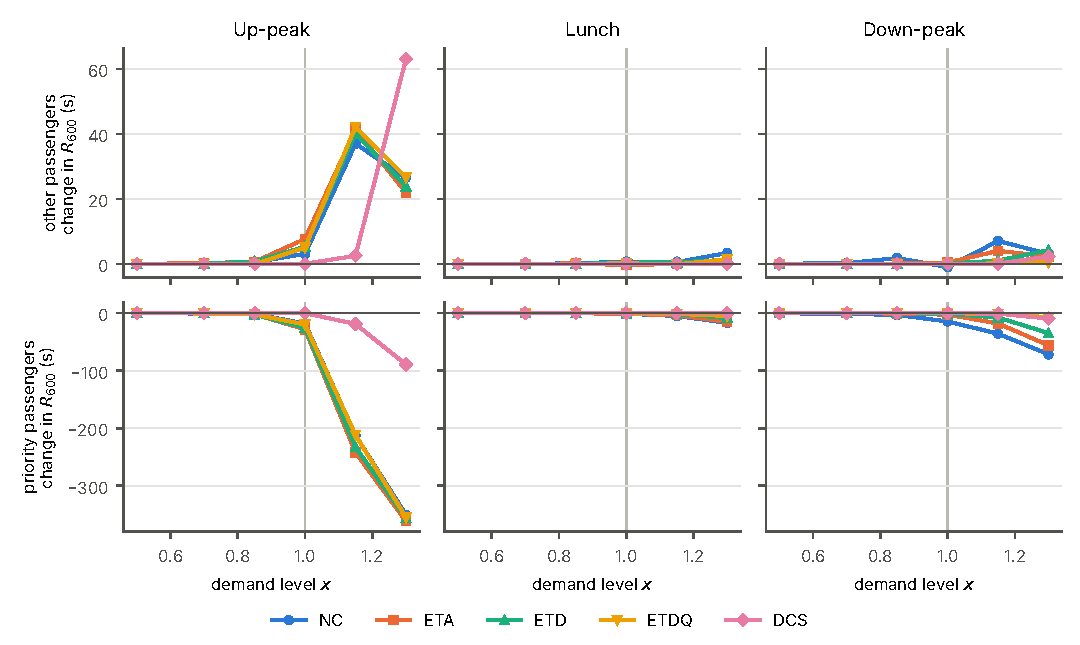
\includegraphics[width=\linewidth]{priority_cost.pdf}
\caption{Priority-first boarding with 15\% simple priority passengers and steady demand, for each standard controller. Top: change in capped average wait for other passengers (above zero means a longer wait). Bottom: change for priority passengers (below zero means a shorter wait). The grey vertical line marks handling capacity.}\label{fig:priority}\end{figure}

\subsection{Destination control and the new priority-aware rule}\label{sec:dcsp}
Table~\ref{tab:dcs} and Figure~\ref{fig:dcs} compare three ways to give priority under destination control. Each is compared with destination control and FCFS boarding.

\emph{Door-only priority does nothing until the system is overloaded.} Up to capacity, priority at the door changes no waiting time by more than 0.2~s, for priority passengers or for others. The reason is simple. A passenger can board only the car they were sent to, and below capacity that car has room for everyone sent to it. When demand rises and falls, the result is the same up to a peak of 115\%. In overload, door-only priority helps priority passengers much less than with call buttons (32.9~s at $x=1.3$, against 122 to 146~s), because a priority passenger must still wait for one fixed car.

\emph{DCS-P1 changes little.} When the controller still counts the delay to all other passengers, it rarely moves a priority passenger to an earlier car. The gain is only slightly larger than with door-only priority (38.6~s against 32.9~s at $x=1.3$).

\emph{DCS-P0 helps priority passengers at every demand level.} When the controller gives a priority passenger the car with the shortest trip, priority passengers wait 5.6~s less at $x=0.5$, 10.2~s less at $x=0.7$, 14.4~s less at $x=0.85$ and 17.8~s less at $x=1$. This is 30\% to 43\% of their waiting time. The gain is statistically clear in all 36 cases at or below capacity. The other passengers pay 0.7, 1.7, 2.6 and 4.1~s. For wheelchair-like passengers the gains are 6.2 to 23.3~s and the costs 0.3 to 2.6~s. This is the only tested way to shorten the wait of priority passengers while the building works normally.

\emph{In overload DCS-P0 is expensive.} At $x=1.15$ the other passengers wait 17.1~s longer for a priority gain of 27.3~s, and at $x=1.3$ they wait 59.5~s longer for a gain of 55.3~s. Each priority passenger then causes extra stops for full cars. With rising and falling demand the cost stays moderate up to a peak of 130\% (12.8~s for a gain of 20.4~s).

\begin{table}[htbp]\centering
\caption{Three ways to give priority under destination control, with 15\% simple priority passengers. Average change in capped average wait $R_{600}$ (s) against destination control with first-come-first-served boarding. Plus means a longer wait.}\label{tab:dcs}
\small\begin{tabular}{@{}lrrrrrr@{}}
\toprule & \multicolumn{2}{c}{Door-only priority} & \multicolumn{2}{c}{DCS-P1 (new)} & \multicolumn{2}{c}{DCS-P0 (new)}\\
Demand & Others & Priority & Others & Priority & Others & Priority\\\midrule
Steady, 50\% & 0.0 & 0.0 & 0.0 & 0.0 & $+0.6$ & $-5.6$\\
Steady, 70\% & 0.0 & 0.0 & 0.0 & 0.0 & $+1.7$ & $-10.2$\\
Steady, 85\% & 0.0 & 0.0 & 0.0 & $-0.1$ & $+2.6$ & $-14.4$\\
Steady, 100\% & 0.0 & 0.0 & 0.0 & $-0.3$ & $+4.1$ & $-17.8$\\
Steady, 115\% & $+0.9$ & $-6.5$ & $+1.8$ & $-9.0$ & $+17.1$ & $-27.3$\\
Steady, 130\% & $+21.8$ & $-32.9$ & $+23.9$ & $-38.6$ & $+59.5$ & $-55.3$\\
\midrule
Rise and fall, peak 100\% & 0.0 & 0.0 & 0.0 & $-0.2$ & $+1.5$ & $-9.7$\\
Rise and fall, peak 115\% & 0.0 & $-0.1$ & $+0.1$ & $-1.3$ & $+3.6$ & $-12.3$\\
Rise and fall, peak 130\% & 0.0 & $-4.3$ & $+2.1$ & $-9.3$ & $+12.8$ & $-20.4$\\
Rise and fall, peak 150\% & $+6.7$ & $-35.3$ & $+11.2$ & $-50.1$ & $+44.3$ & $-65.3$\\
\bottomrule\end{tabular}
\end{table}

\begin{figure}[htbp]\centering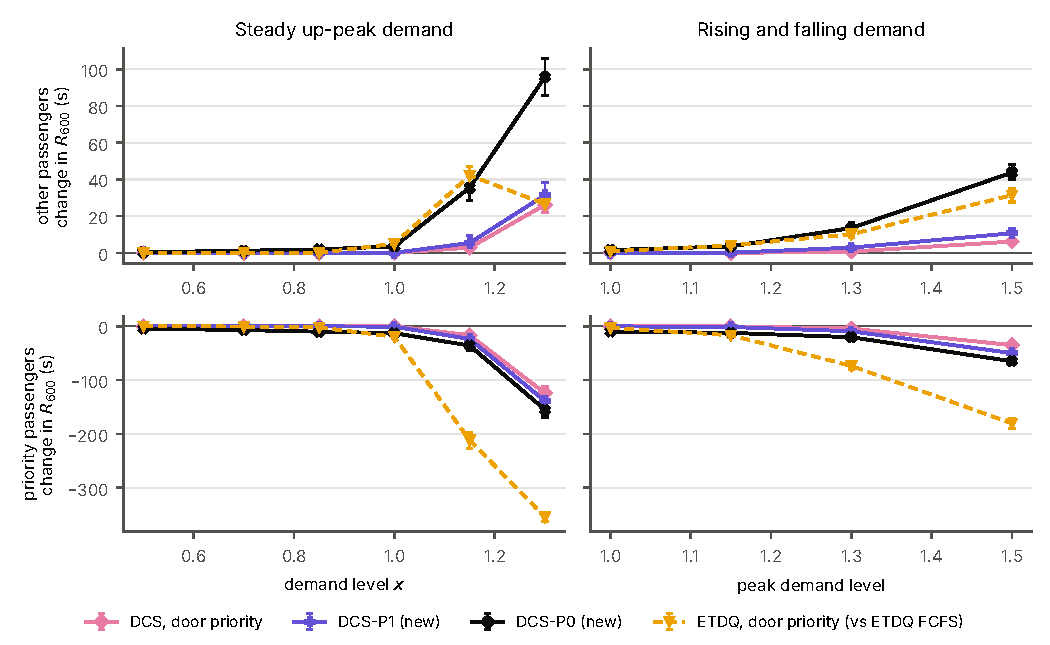
\includegraphics[width=\linewidth]{dcs_priority.pdf}
\caption{Priority under destination control in up-peak traffic, with 15\% simple priority passengers. Left: steady demand. Right: rising and falling demand. Top: change for other passengers. Bottom: change for priority passengers. The dashed line shows the best call-button controller (ETDQ) with door priority for comparison.}\label{fig:dcs}\end{figure}

\subsection{Do the two measures rank controllers in the same order?}\label{sec:disagreement}
Yes. There are 660 comparisons (66 situations $\times$ 10 pairs of standard controllers). The served-only average and the capped average $R_{600}$ give opposite answers in only one, and that one is not clear: in building B2, lunch traffic, $x=1.3$, the NC and ETA controllers differ by less than 0.5~s on both measures. The capped average itself separates the two controllers clearly in 566 of the 660 comparisons.

The cap matters a little more than who is counted. With a cap of 300~s the served-only average disagrees in ten comparisons, all above capacity and none clear (Table~\ref{tab:disc}). One reason for this good agreement is the test plan. People keep arriving after the counted period and every counted passenger is watched for 900~s, so even at $x=1.3$ in up-peak traffic 95\% of counted passengers are served. The \emph{size} of the served-only average is still wrong in overload: at $x=1.3$ in up-peak it is 419~s against 352~s for the capped average.

\begin{table}[htbp]\centering
\caption{Number of controller pairs for which two measures give opposite answers. In brackets: clear disagreements. ``Served-only'' is the usual average over served passengers; $R_{600}^{\mathrm{s}}$ is the capped average over served passengers only.}\label{tab:disc}
\small\begin{tabular}{@{}lrrrrr@{}}
\toprule Demand & Pairs & Served-only & $R_{600}^{\mathrm{s}}$ & Served-only & $R_{300}$\\
 & & vs $R_{600}$ & vs $R_{600}$ & vs $R_{300}$ & vs $R_{900}$\\\midrule
Steady, 50\% & 90 & 0 (0) & 0 (0) & 0 (0) & 0 (0)\\
Steady, 70\% & 90 & 0 (0) & 0 (0) & 0 (0) & 0 (0)\\
Steady, 85\% & 90 & 0 (0) & 0 (0) & 0 (0) & 0 (0)\\
Steady, 100\% & 90 & 0 (0) & 0 (0) & 0 (0) & 0 (0)\\
Steady, 115\% & 90 & 0 (0) & 0 (0) & 3 (0) & 3 (0)\\
Steady, 130\% & 90 & 1 (0) & 0 (0) & 6 (0) & 7 (0)\\
\midrule
Rise and fall, peak 100\% & 30 & 0 (0) & 0 (0) & 0 (0) & 0 (0)\\
Rise and fall, peak 115\% & 30 & 0 (0) & 0 (0) & 0 (0) & 0 (0)\\
Rise and fall, peak 130\% & 30 & 0 (0) & 0 (0) & 0 (0) & 0 (0)\\
Rise and fall, peak 150\% & 30 & 0 (0) & 0 (0) & 1 (0) & 1 (0)\\
\bottomrule\end{tabular}
\end{table}

\section{Discussion}\label{sec:discussion}

\subsection{Advice on boarding priority}
Lift systems are designed to work below their handling capacity \cite{cibse2025,iso8100}. In that range, every waiting person fits into the next car. Three practical points follow.

\emph{With call buttons, priority at the door is safe to adopt.} It costs other passengers almost nothing in normal operation and a few seconds at capacity. It pays off in busy periods: with a demand peak of 115\% of capacity, priority passengers save about 19~s and others lose about 4~s.

\emph{With destination control, priority at the door is not enough.} It has no effect in normal operation and a weak effect in overload. If priority passengers should really be served sooner, the controller must use the priority label when it chooses the car. The DCS-P0 rule does this. In normal operation it cuts the wait of priority passengers by about a third, and others lose 1 to 4~s. In heavy overload it becomes expensive for the others. A sensible design would use DCS-P0 in normal operation and return to DCS-P1 or door-only priority when the controller detects overload. Testing such a switching rule is future work.

\emph{Space matters more than order.} Passengers who need three places and more time reduce the capacity of the lift group for everyone. At capacity this costs all passengers about 22~s, while the boarding rule costs other passengers about 3~s. Lift planning for accessible buildings should therefore count such passengers when it calculates handling capacity.

\subsection{Advice on measuring waiting time}
In our tests the usual served-only average ranks controllers in the same order as the capped average of all passengers. This holds when the test follows two rules: people keep arriving after the counted period, and every counted passenger is watched for a fixed minimum time. A study that stops watching when arrivals stop leaves out more people and may not be as safe. We advise that studies which include demand at or above capacity should (i) watch every counted passenger for a stated minimum time, (ii) report a capped average with a cap no longer than that time, together with the share of passengers served, and (iii) state the cap. In deep overload a capped average hides part of a cost, because many waits are already at the cap; the results at $x=1.3$ should be read with this in mind.

\subsection{Limits of this study}
\begin{itemize}[itemsep=2pt]
\item The controllers are clear textbook versions and one queue-aware version. They are not commercial products, and we did not build the learning controllers from the literature \cite{crites1998,wan2024,wang2021}.
\item The buildings are simple: one lobby, the same number of people on each floor, no zones. Arrivals are single people, not groups.
\item Speeds and door times are typical design values. The space (three places) and time (three times normal) of the wheelchair-like passenger are assumptions. No data from a real building were used.
\item We assume that the priority label is always correct and that other passengers accept the boarding order.
\item DCS-P0 and DCS-P1 are two fixed settings. Values in between, and a rule that changes with demand, were not tested.
\item The capped average describes waits up to 600~s. It does not say how long the unserved people finally wait.
\item The intervals are not corrected for the many comparisons.
\end{itemize}

\section{Conclusions}\label{sec:conclusions}
We built a lift simulator that works in seconds and agrees with the classical round-trip formula within 2\%. With it we compared five group controllers, two boarding rules, two kinds of priority passenger and a new priority-aware destination control rule in 31,680 runs with identical passengers.

With call buttons, priority-first boarding costs other passengers almost nothing below handling capacity (at most 3.3~s in any case) and about 2~s at capacity, where priority passengers gain about 9~s. In overload the gain is large (81~s at 115\% of capacity) and the cost moderate (14~s). The same holds for wheelchair-like passengers, but their need for space and time lowers capacity for everyone, and this effect is several times larger than the effect of the boarding order.

With destination control, priority at the door has no effect in normal operation. The new rule DCS-P0, which uses the priority label when it chooses the car, cuts the wait of priority passengers by 30\% to 43\% in normal operation at a cost of 1 to 4~s for others, but it is expensive in heavy overload.

The usual served-only average and the capped average of all passengers rank the controllers in the same order in 659 of 660 comparisons. The simulator, the test plan and all results are public for others to use.
